%% Neurocomputing submission. Compile with XeLaTeX (Indic scripts):  latexmk -xelatex main.tex
%% Numbers and tables are generated from the repository by:  python3 paper/make_numbers.py
\documentclass[preprint,12pt]{elsarticle}

\usepackage{fontspec}
\usepackage{amsmath,amssymb}
\usepackage{booktabs,multirow,array,tabularx}
\usepackage{graphicx}
\usepackage[table]{xcolor}
\usepackage{hyperref}
\usepackage{lineno}
\usepackage{algorithm}
\usepackage{algpseudocode}
\hypersetup{colorlinks=true,linkcolor=blue!50!black,citecolor=blue!50!black,urlcolor=blue!50!black}

\newfontfamily\devanagari{Noto Sans Devanagari}[Script=Devanagari]
\newfontfamily\bengali{Noto Sans Bengali}[Script=Bengali]
\newfontfamily\telugu{Noto Sans Telugu}[Script=Telugu]
\newcommand{\pending}[1]{\colorbox{yellow!60}{\strut\hspace{1.6em}}}
% generated by paper/make_numbers.py — do not edit
\newcommand{\ACalls}{3,074}
\newcommand{\ACallsPerQ}{3.1}
\newcommand{\ACitedAll}{86.2}
\newcommand{\ACitedRecall}{92.5}
\newcommand{\ACorrect}{998}
\newcommand{\AIncorrect}{0}
\newcommand{\ALenient}{99.9}
\newcommand{\ANumeric}{97.4}
\newcommand{\APartial}{2}
\newcommand{\AStrict}{99.8}
\newcommand{\FTBaseClosed}{\pending{}}
\newcommand{\FTBaseOracle}{\pending{}}
\newcommand{\FTBaseRag}{\pending{}}
\newcommand{\FTDeltaClosed}{\pending{}}
\newcommand{\FTDeltaOracle}{\pending{}}
\newcommand{\FTDeltaRag}{\pending{}}
\newcommand{\FTGoldInCtxRag}{\pending{}}
\newcommand{\FTPending}{1}
\newcommand{\FTSEBaseClosed}{\pending{}}
\newcommand{\FTSEBaseOracle}{\pending{}}
\newcommand{\FTSEBaseRag}{\pending{}}
\newcommand{\FTSETunedClosed}{\pending{}}
\newcommand{\FTSETunedOracle}{\pending{}}
\newcommand{\FTSETunedRag}{\pending{}}
\newcommand{\FTTopLang}{\pending{}}
\newcommand{\FTTopLangDelta}{\pending{}}
\newcommand{\FTTunedClosed}{\pending{}}
\newcommand{\FTTunedOracle}{\pending{}}
\newcommand{\FTTunedRag}{\pending{}}
\newcommand{\FTVerbClosed}{\pending{changes}}
\newcommand{\FTVerbOracle}{\pending{changes}}
\newcommand{\FTVerbRag}{\pending{changes}}
\newcommand{\FTXLBaseClosed}{\pending{}}
\newcommand{\FTXLBaseOracle}{\pending{}}
\newcommand{\FTXLBaseRag}{\pending{}}
\newcommand{\FTXLTunedClosed}{\pending{}}
\newcommand{\FTXLTunedOracle}{\pending{}}
\newcommand{\FTXLTunedRag}{\pending{}}
\newcommand{\MaxDocWords}{17k}
\newcommand{\MinDocWords}{12k}
\newcommand{\NCrossDoc}{710}
\newcommand{\NCrossLang}{100}
\newcommand{\NCrossSec}{180}
\newcommand{\NDev}{49}
\newcommand{\NDocs}{50}
\newcommand{\NDropped}{0}
\newcommand{\NFacts}{6,315}
\newcommand{\NFixed}{0}
\newcommand{\NFreeFacts}{4,881}
\newcommand{\NPages}{3,444}
\newcommand{\NSharedFacts}{0}
\newcommand{\NTest}{1,000}
\newcommand{\NTestFacts}{1,434}
\newcommand{\NTrain}{533}
\newcommand{\NTrainDev}{582}
\newcommand{\NTrainFacts}{804}
\newcommand{\NWithinSec}{10}
\newcommand{\NWords}{675,913}
\newcommand{\NWordsK}{676k}
\newcommand{\NWritten}{582}
\newcommand{\RAllTen}{63.8}
\newcommand{\RBestLang}{Bengali}
\newcommand{\RBestLangV}{84.7}
\newcommand{\RCDTen}{66.3}
\newcommand{\RCSTen}{85.0}
\newcommand{\RFactTen}{80.8}
\newcommand{\RWorstLang}{Punjabi}
\newcommand{\RWorstLangV}{55.6}
\newcommand{\RXLLFTen}{59.0}
\newcommand{\RXLTen}{4.0}
\newcommand{\TrainCheck}{Training questions were written under the same protocol, each was re-checked by its writer against the verbatim evidence, and all passed the same automatic checks for fact presence, hop-type consistency, value leakage and script purity.}

\makeatletter\newcommand{\tabin}[1]{\@@input generated/#1.tex }\makeatother

\journal{Neurocomputing}

\begin{document}

\begin{frontmatter}

\title{Retrieval-augmented multi-hop question answering over enterprise policies in eight Indian languages:\\ a contamination-free benchmark, an agentic baseline and retrieval-aware fine-tuning}

\author{Angshul Majumdar}
\ead{angshul@iiitd.ac.in}
\affiliation{organization={Indraprastha Institute of Information Technology Delhi},
            city={New Delhi},
            postcode={110020},
            country={India}}

\begin{abstract}
Enterprise question answering in multilingual organisations requires a system to locate several clauses spread across long policy manuals, sometimes written in different languages, and to combine them through comparison or arithmetic. Existing Indic question-answering resources are built from short, mostly translated passages with single-span answers and cannot measure this ability. We introduce a benchmark built on a controlled corpus of \NDocs{} human-resources policy manuals of a single fictional company, written natively in Bengali, Hindi, Kannada, Marathi, Odia, Punjabi, Tamil and Telugu (\NWords{} words, \NPages{} pages). Every manual is accompanied by a fact ledger of verbatim-grounded facts (\NFacts{} in total), from which we construct \NTest{} multi-hop test questions spanning cross-document, cross-section and cross-language reasoning, together with a training split whose facts are disjoint from the test set. We study three systems on this resource: a lexical retriever designed for Indic morphology, an agentic retrieval-augmented generation (RAG) pipeline that plans language-specific queries, and a compact open model adapted with retrieval-aware LoRA fine-tuning. Single-query retrieval places all required evidence in the top ten passages for \RAllTen\% of questions but for only \RXLTen\% of cross-language questions; issuing one query per language raises the latter to \RXLLFTen\%. The agentic pipeline answers \AStrict\% of questions correctly. Retrieval-aware fine-tuning of a 1B-parameter model \FTVerbRag{} its RAG accuracy from \FTBaseRag\% to \FTTunedRag\%. The corpus, ledgers, questions, systems and evaluation code are released.
\end{abstract}

\begin{keyword}
Retrieval-augmented generation \sep Multi-hop question answering \sep Multilingual NLP \sep Indian languages \sep Parameter-efficient fine-tuning \sep Benchmark dataset
\end{keyword}

\end{frontmatter}

\linenumbers

%% ==========================================================================
\section{Introduction}
\label{sec:intro}

Retrieval-augmented generation (RAG) has become the standard way of grounding large language models (LLMs) in organisational knowledge \cite{lewis2020rag,gao2023ragsurvey}. In an enterprise deployment the knowledge base is a set of long, structured documents (policies, manuals, contracts) and the questions users ask are rarely answered by a single sentence. An employee asking how long she must wait after confirmation before becoming eligible for a welfare benefit needs the probation clause from one manual and the eligibility clause from another, and must subtract one duration from the other. In a multilingual organisation such as a pan-Indian company, the two manuals may be maintained by different regional offices in different languages.

Three properties of this setting are poorly covered by existing resources. First, the evidence is distributed: the answer depends on two or more clauses located in different sections or documents, so success requires multi-hop retrieval and composition rather than span extraction \cite{yang2018hotpotqa,trivedi2022musique}. Second, the documents are long and native: Indian enterprise documents are written in the regional language with its own terminology, numeral system and conventions, whereas most Indic QA data are translated from English or drawn from short encyclopaedic passages \cite{lewis2020mlqa,doddapaneni2023indicxtreme}. Third, the evaluation must be free of contamination: when the facts of a benchmark are present in pre-training corpora, a model can answer from memory, and the benchmark no longer measures retrieval and reading \cite{sainz2023contamination}.

This paper addresses these gaps with four artefacts and an evaluation protocol that ties them together.
\begin{enumerate}
\item \textbf{A benchmark corpus and question set.} \NDocs{} HR-policy manuals of a single fictional company, written natively in eight Indian languages and totalling \NWords{} words, each paired with a fact ledger whose entries carry a verbatim evidence sentence, a section and a page. On this corpus we build \NTest{} multi-hop questions with short and long reference answers and fact-level provenance, including \NCrossLang{} cross-language questions over deliberately confusable topic pairs, and a training split whose facts are disjoint from the test set (Section~\ref{sec:dataset}).
\item \textbf{A RAG system before fine-tuning.} A section-aware chunker and a hybrid lexical retriever that fuses word-level and character-level BM25 with reciprocal rank fusion, together with an agentic pipeline that decomposes each question into per-fact queries issued in the language of the document most likely to contain the fact (Section~\ref{sec:method}).
\item \textbf{A retrieval-aware fine-tuned reader.} A compact open model (Gemma~3, 1B parameters \cite{gemma3}) adapted with LoRA \cite{hu2022lora} on training questions whose gold passages are mixed with hard distractors drawn from the retriever, following the retrieval-augmented fine-tuning paradigm \cite{zhang2024raft}.
\item \textbf{A RAG system after fine-tuning}, evaluated under the same protocol as the base system.
\end{enumerate}
The evaluation protocol separates retrieval from reading through three conditions (closed-book, retrieved context and oracle context) and reports fact-level evidence recall, automatic numeric correctness and judged correctness per language and per hop type (Section~\ref{sec:experiments}).

Our experiments yield three findings. (i) Lexical retrieval tuned for Indic scripts is strong within a language but collapses across languages: the evidence for a cross-language question is fully retrieved by a single query in only \RXLTen\% of cases, against \RAllTen\% overall, and per-language querying recovers most of the gap. (ii) An agentic pipeline that plans language-specific queries reaches \AStrict\% strict accuracy, showing that the benchmark is fully answerable from its corpus and that the gap left by single-query retrieval is a planning problem. (iii) Retrieval-aware fine-tuning transfers this behaviour to a small model that can be deployed on commodity hardware.

%% ==========================================================================
\section{Related work}
\label{sec:related}

\paragraph{Multi-hop question answering}
HotpotQA \cite{yang2018hotpotqa}, 2WikiMultiHopQA \cite{ho2020twowiki} and MuSiQue \cite{trivedi2022musique} established multi-hop QA over Wikipedia, with MuSiQue constructing questions bottom-up from single-hop components to prevent shortcut reasoning. These datasets are English-only and built on short encyclopaedic paragraphs whose facts are widely present in pre-training data. Our benchmark adopts the compositional, fact-first construction of MuSiQue but applies it to long, native, non-public documents in eight languages.

\paragraph{Multilingual and Indic QA}
MLQA \cite{lewis2020mlqa}, XQuAD \cite{artetxe2020xquad} and TyDi QA \cite{clark2020tydiqa} evaluate cross-lingual and typologically diverse extractive QA; XOR QA \cite{asai2021xorqa} adds open-retrieval across languages. For Indian languages, IndicXTREME \cite{doddapaneni2023indicxtreme} and the IndicNLP suite \cite{kakwani2020indicnlpsuite} provide broad task coverage, and large parallel corpora such as Samanantar \cite{ramesh2022samanantar} support translation-based transfer. These resources mostly contain single-span answers in short contexts, often translated from English. Our corpus is written natively per language, keeps native numeral systems, and requires composing facts across long documents and across languages.

\paragraph{Retrieval-augmented generation}
RAG \cite{lewis2020rag} and Fusion-in-Decoder \cite{izacard2021fid} condition generation on retrieved passages; dense retrievers \cite{karpukhin2020dpr,khattab2020colbert} and multilingual embedding models such as BGE-M3 \cite{chen2024bgem3} complement lexical scoring \cite{robertson2009bm25}, and reciprocal rank fusion \cite{cormack2009rrf} is a robust way to combine ranked lists. Iterative and agentic schemes interleave retrieval with reasoning: IRCoT \cite{trivedi2023ircot}, self-ask \cite{press2023selfask}, ReAct \cite{yao2023react} and Self-RAG \cite{asai2024selfrag}. Our agentic baseline belongs to this family and specialises query planning to the language of each target document.

\paragraph{Adapting readers to retrieval}
Parameter-efficient methods such as LoRA \cite{hu2022lora} and QLoRA \cite{dettmers2023qlora} make domain adaptation of LLMs affordable. Retrieval-augmented fine-tuning (RAFT) \cite{zhang2024raft} trains a reader on questions paired with gold and distractor documents so that it learns to ignore irrelevant context. We apply this idea to multilingual multi-hop reading, with distractors taken from the benchmark's own retriever so that they are the hardest negatives the deployed system will encounter.

\paragraph{Evaluation with LLM judges}
LLM-as-a-judge evaluation correlates well with human preference for open-ended answers \cite{zheng2023judge}. We pair judged correctness with an automatic numeric criterion that requires no model, and with fact-level evidence metrics that require no generation at all.

%% ==========================================================================
\section{The benchmark}
\label{sec:dataset}

\subsection{Design principles}
The benchmark is built around four principles. \emph{Contamination control:} all documents describe a single fictional company, Suryodaya Integrated Solutions Pvt.\ Ltd., so none of the facts can be known before reading the corpus. \emph{Native authorship:} each manual is written directly in its language with the terminology, register and numeral conventions of that language, not translated. \emph{Verifiable grounding:} every fact used by a question is recorded in a ledger together with the verbatim sentence that states it, its section and its page. \emph{Compositionality:} every question requires at least two ledger facts and an explicit operation on them.

\subsection{Corpus}
Table~\ref{tab:dataset} summarises the corpus. The \NDocs{} manuals cover the employee life cycle: recruitment, onboarding, probation, compensation and payroll, leave, attendance and overtime, travel, remote work, performance and promotion, training, discipline and inquiries, grievances, prevention of sexual harassment, whistle-blowing, benefits, loans, retirement funds, workplace safety, IT use and separation. Manuals range from \MinDocWords{} to \MaxDocWords{} words and are organised in numbered sections and subsections, with tables, worked examples and page boundaries. Bengali, Devanagari, Gurmukhi and Odia manuals predominantly use native digits, whereas Tamil, Telugu and Kannada manuals predominantly use Western digits, mirroring regional practice; a system must therefore normalise numerals before it can compare figures.

\begin{table}[t]
\centering
\caption{Corpus and question statistics. Facts are ledger entries with verbatim evidence. Training counts include the development split.}
\label{tab:dataset}
\small
\begin{tabular}{llrrrrr}
\toprule
Language & Script & Docs & Words & Facts & Test Qs & Train Qs \\
\midrule
\tabin{table_dataset}
\bottomrule
\end{tabular}
\end{table}

\paragraph{Topic-collision pairs}
Five pairs of manuals in different languages share a topic but no content: recruitment (Bengali, Telugu), travel (Hindi, Telugu), separation (Bengali, Telugu), discipline (Hindi, Kannada) and training (Hindi, Kannada). A retriever that matches the topic of a question rather than the specific fact will return the wrong manual; the cross-language questions are built on these pairs.

\subsection{Fact ledgers}
Each manual has a ledger of structured facts $f=(s,a,v,u,\sigma,p,e)$ with subject $s$, aspect $a$, value $v$, unit $u$, section $\sigma$, page $p$ and evidence $e$, where $e$ is a verbatim substring of the manual. The corpus contains \NFacts{} facts. Questions reference facts by $(\text{language},\text{document},s,a)$, so every reference answer can be traced to the exact sentences that justify it.

\subsection{Questions}
A question $q$ is defined by its supporting facts $F_q=\{f_1,f_2\}$ and an operation over their values (difference, ratio, sum, threshold test, eligibility under both rules, date arithmetic, or selection of the stricter or looser limit). Four hop types are distinguished:
\begin{itemize}
\item \emph{cross-document} (\NCrossDoc{} test questions): $f_1$ and $f_2$ come from two manuals in the same language;
\item \emph{cross-section} (\NCrossSec{}): from two top-level sections of one manual;
\item \emph{cross-language} (\NCrossLang{}): from two manuals of a topic-collision pair, with the question written in one of the two languages;
\item \emph{within-section} (\NWithinSec{}): two distinct facts of one section.
\end{itemize}
Each question carries a short answer (a number with its unit, a yes/no decision with the decisive figure, a date or a short phrase), a two-to-four sentence answer that states the facts with their section numbers and the reasoning, the source sections and the supporting facts. Questions are written so that they do not state the values they test: a rule is described precisely (``the notice period for executive-grade staff'') and must be looked up. Hypothetical scenario figures (a salary, a joining date, a number of dependants) are allowed where they make the computation concrete. Figure~\ref{fig:dataset} shows the distribution of test questions, and two examples follow.

\begin{figure}[t]
\centering
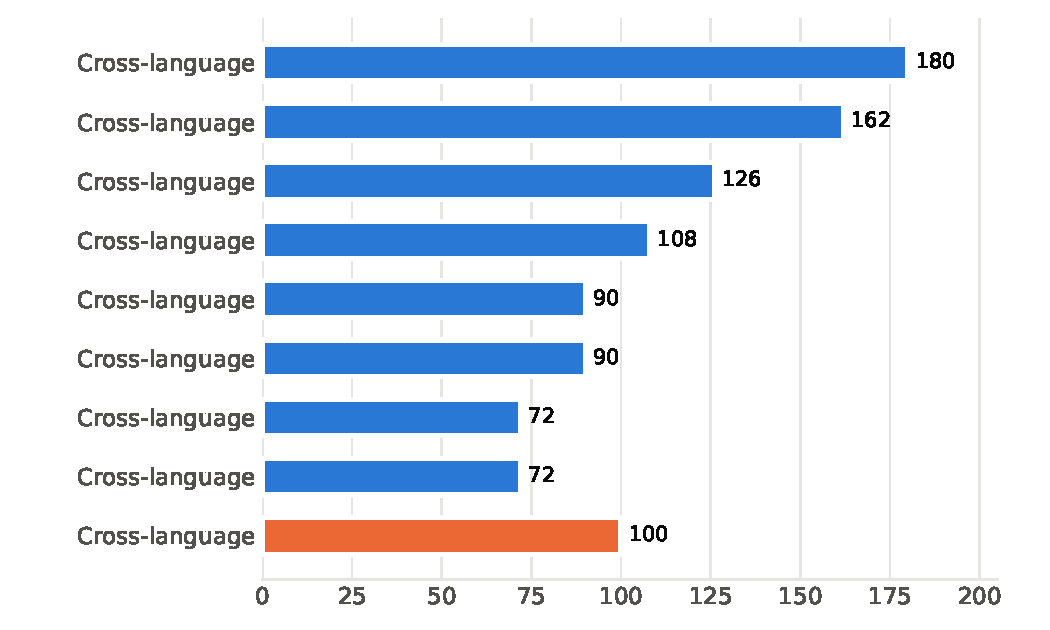
\includegraphics[width=0.8\linewidth]{figures/fig1_dataset.pdf}
\caption{Test questions per language. Cross-language questions require one fact from each of two languages.}
\label{fig:dataset}
\end{figure}

\paragraph{Example 1 (Hindi, cross-document)}
{\devanagari कार्यपालक-स्तर के कर्मी की परिवीक्षा-अवधि कितनी है, और कल्याण कोष के लाभों के लिए न्यूनतम कितनी सेवा-अवधि आवश्यक है? परिवीक्षा पूरी होते ही स्थायी हुए कर्मी को इन लाभों के लिए स्थायीकरण के बाद कितना अतिरिक्त समय प्रतीक्षा करनी होगी?}
\emph{(What is the probation period of an executive, what minimum service is needed for the welfare-fund benefits, and how much longer must an employee confirmed at the end of probation wait?)} Short answer: {\devanagari ६ माह अतिरिक्त} (six more months), from the probation rules (\S4.1) and the benefits manual (\S4.3).

\paragraph{Example 2 (Bengali--Telugu, cross-language)}
{\bengali বাংলা নিয়োগ নির্দেশিকা অনুযায়ী সম্পূর্ণ পূর্বতন কর্মজীবন যাচাই প্রক্রিয়া সম্পন্ন করার সময়সীমা কত, এবং তেলুগু নির্দেশিকায় উল্লিখিত নেপথ্য ধৃবীকরণ ({\telugu నేపథ్య ధృవీకరణ})-র প্রমিত সময়সীমার তুলনায় তা কত কার্যদিবস বেশি?}
\emph{(How long is the full background verification under the Bengali recruitment manual, and how many working days longer is it than the standard background-verification time in the Telugu manual?)} Short answer: 14 working days, 4 more than Telugu's 10 (Bengali \S16.8, Telugu \S8.3).

\subsection{Construction and verification}
The corpus and questions were produced with an LLM-assisted, ledger-first protocol designed for verifiability. Manuals were authored natively per language from a common design specification of the company's policy structure. Ledgers were extracted from the finished manuals, and each entry was retained only if its evidence sentence occurs verbatim in the manual. Questions were then composed from pairs of ledger facts by model instances that saw only the facts and their evidence, and were checked automatically for (i) the presence of each supporting fact, (ii) consistency between the declared hop type and the facts' documents and sections, (iii) absence of tested values from the question text after numeral normalisation, and (iv) script and language purity. Every answer was then judged by independent model instances against the verbatim evidence. Questions or manual passages flagged during judging were revised until no reference was disputed, and an end-to-end consistency pass removed contradictions between and within manuals so that each fact has exactly one reading.

\subsection{Training split}
\label{sec:train}
Of the \NFacts{} ledger facts, \NTestFacts{} support test questions; a training split of \NTrainDev{} questions (\NTrain{} training, \NDev{} development) is built from the remaining \NFreeFacts{}. It covers all eight languages, all four hop types and all five cross-language topic pairs (Table~\ref{tab:dataset}), with a larger share of cross-language questions than the test set so that cross-script alignment is well represented during training. The two splits share manuals but no facts (\NSharedFacts{} shared facts), so fine-tuning can teach a model how to read and combine policy clauses without exposing any fact that is tested. \TrainCheck{}

%% ==========================================================================
\section{Methods}
\label{sec:method}

\subsection{Section-aware chunking}
Manuals are segmented along their own heading structure. A chunk never crosses a section boundary, holds at most 220 words, and carries its document title and full heading path (for example ``7. Notice period $>$ 7.1 Grade-wise length''), which disambiguates otherwise similar passages across manuals. The corpus yields 5,507 chunks.

\subsection{Hybrid lexical retrieval for Indic scripts}
\paragraph{Normalisation and tokenisation} All Indic digit blocks are mapped to ASCII digits. Word tokens are maximal runs of word characters \emph{including} the Indic vowel signs, viramas and joiners (Unicode ranges U+0900--U+0963, U+0966--U+0D7F, U+200C, U+200D). This detail matters: the default regular-expression word class splits Indic words at every dependent vowel sign, fragmenting terms such as {\devanagari परिवीक्षा} into meaningless pieces. With the corrected tokeniser the share of questions whose evidence is fully retrieved in the top ten doubles relative to the default class (from 30\% to \RAllTen\%).

\paragraph{Scoring} Two BM25 indexes \cite{robertson2009bm25} ($k_1=1.4$, $b=0.75$) are built over word tokens and over character 4-grams of the normalised text. The character view captures inflection, agglutination and compounding, which are pervasive in Dravidian languages and frequent in Indo-Aryan ones. For a query $q$ the two ranked lists $L_w$ and $L_c$ are fused by reciprocal rank fusion \cite{cormack2009rrf},
\begin{equation}
\mathrm{RRF}(d)=\sum_{L\in\{L_w,L_c\}} \frac{1}{k+\mathrm{rank}_L(d)},\qquad k=60,
\end{equation}
and an optional third list from multilingual dense embeddings (BGE-M3 \cite{chen2024bgem3}) can be added in the same way. Searches can be restricted to a language or to a document.

\subsection{Agentic RAG}
\label{sec:agentic}
Figure~\ref{fig:pipeline} outlines the agentic pipeline. For a question $q$ the agent (i) decomposes $q$ into the facts it needs, (ii) writes for each fact a keyword query in the language of the manual most likely to contain it, using that manual's own terminology, and restricts the search to that language, (iii) reads the retrieved passages and their neighbours, (iv) answers only from the passages, citing the chunk identifiers it used, and (v) re-plans for any fact it reports missing. The language-targeted queries are what allow the pipeline to cross the language boundary that defeats single-query retrieval. Algorithm~\ref{alg:agentic} gives the procedure.

\begin{figure}[t]
\centering
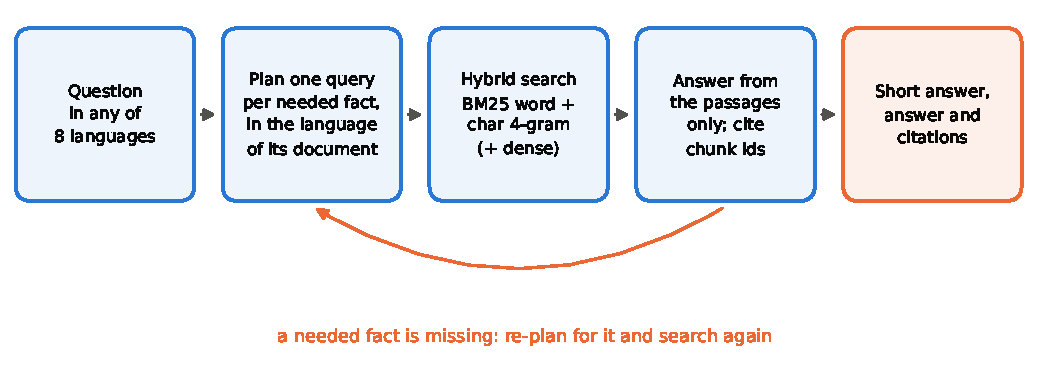
\includegraphics[width=\linewidth]{figures/fig4_pipeline.pdf}
\caption{Agentic RAG: per-fact, language-targeted query planning; hybrid retrieval; grounded answering with citations; re-planning for missing facts.}
\label{fig:pipeline}
\end{figure}

\begin{algorithm}[t]
\caption{Language-targeted agentic RAG}
\label{alg:agentic}
\begin{algorithmic}[1]
\Require question $q$, retriever $\mathcal{R}$, reader $\mathcal{M}$, rounds $T$, budget $K$
\State $\mathcal{C}\gets$ top-$\lceil K/2\rceil$ of $\mathcal{R}(q)$ \Comment{the question's own evidence}
\For{$t=1,\dots,T$}
  \State $\{(q_j,\ell_j)\}\gets \mathcal{M}.\textsc{Plan}(q,\text{missing})$ \Comment{one query per needed fact, with its language}
  \State $\mathcal{C}\gets \mathcal{C}\cup \textsc{RoundRobin}\big(\{\mathcal{R}(q_j;\ \text{lang}=\ell_j)\}_j\big)$ up to $K$ passages
  \State $(\hat a,\text{cites},\text{missing})\gets \mathcal{M}.\textsc{Answer}(q,\mathcal{C})$
  \If{$\text{missing}=\emptyset$} \textbf{break} \EndIf
\EndFor
\State \Return $\hat a$, cites
\end{algorithmic}
\end{algorithm}

\subsection{Retrieval-aware fine-tuning of a compact reader}
\label{sec:ft}
The agentic results show that the benchmark is answerable when the reader plans well and reads carefully. To transfer this capability to a model small enough for on-premise deployment, we fine-tune Gemma~3 (1B, instruction-tuned) \cite{gemma3} with LoRA \cite{hu2022lora} in the RAFT style \cite{zhang2024raft}. Each training question $q$ with gold chunks $G_q$ (the chunks containing the evidence of its supporting facts) is paired with a context
\begin{equation}
\mathcal{C}_q = \pi\big(G_q \cup D_q\big),\qquad D_q\subset \mathcal{R}(q)\setminus G_q,\quad |\mathcal{C}_q|=K,
\end{equation}
where $D_q$ are the highest-ranked non-gold chunks returned by the benchmark's own retriever (hard distractors) and $\pi$ is a random permutation. The target is the reference short answer followed by the reference explanation with section citations, and the loss is the token-level cross-entropy on the target only,
\begin{equation}
\mathcal{L}(\theta)=-\sum_{q}\sum_{t\in y_q}\log p_{\theta_0+\Delta\theta}\big(y_{q,t}\mid \mathcal{I},\mathcal{C}_q,q,y_{q,<t}\big),\qquad \Delta W=BA,\ \ \mathrm{rank}(BA)=r,
\end{equation}
with the base weights $\theta_0$ frozen and low-rank updates on all attention and feed-forward projections. Because training facts are disjoint from test facts, the model cannot improve by memorising answers; it can improve only by learning to locate the relevant clauses among distractors in eight scripts, to align terminology across languages, to normalise numerals and to carry out the required operation.

\subsection{Evaluation protocol}
\label{sec:protocol}
Every system answers all \NTest{} test questions under three conditions: \emph{closed-book} (no passages), which measures what can be answered without the corpus; \emph{RAG}, with the top-$K$ passages retrieved for the question; and \emph{oracle}, with the gold passages mixed with retrieved distractors to $K$ passages, which isolates reading from retrieval. We use $K=6$. Four metrics are reported per question language, for the cross-language set and per hop type:
\begin{itemize}
\item \emph{Evidence recall}: fact recall@$k$ (share of supporting facts with a gold chunk in the top $k$) and all-facts@$k$ (share of questions with every supporting fact retrieved).
\item \emph{Numeric match}: every number in the reference short answer appears in the system's answer, after numeral normalisation. This criterion needs no model.
\item \emph{Short-answer exactness}: the set of numbers in the system's short answer equals that of the reference.
\item \emph{Judged accuracy}: correct, partial or incorrect according to a judge that compares the system answer with the reference and the evidence \cite{zheng2023judge}.
\end{itemize}

%% ==========================================================================
\section{Experiments}
\label{sec:experiments}

\subsection{Retrieval}
Table~\ref{tab:retrieval} reports evidence recall for single-query retrieval, using the raw question as the query over all 5,507 chunks, and Figure~\ref{fig:retrieval} summarises the all-facts@10 results. Cross-section questions are the easiest (\RCSTen\% all-facts@10): both facts live in one manual whose title and headings match the question. Cross-document questions fall to \RCDTen\%. Cross-language questions collapse to \RXLTen\%: the lexical signal of the question points to the manual in its own language, and the partner manual, written in another script, is never reached. Restricting retrieval to each fact's language and interleaving the results raises cross-language all-facts@10 to \RXLLFTen\%, which motivates the language-targeted planning of the agentic pipeline.

\begin{table}[t]
\centering
\caption{Single-query evidence recall over the full index (5,507 chunks).}
\label{tab:retrieval}
\footnotesize\setlength{\tabcolsep}{4.5pt}
\begin{tabular}{lrrrrrrr}
\toprule
& & \multicolumn{3}{c}{Fact recall@$k$} & \multicolumn{3}{c}{All facts@$k$} \\
\cmidrule(lr){3-5}\cmidrule(lr){6-8}
Questions & $n$ & 1 & 5 & 10 & 5 & 10 & 20 \\
\midrule
\tabin{table_retrieval}
\bottomrule
\end{tabular}
\end{table}

\begin{figure}[t]
\centering
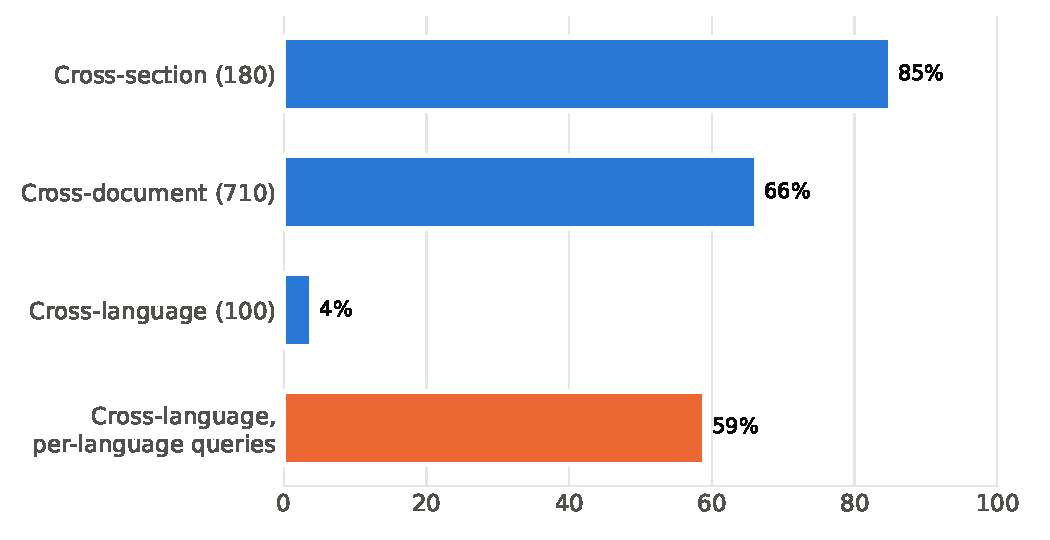
\includegraphics[width=0.78\linewidth]{figures/fig2_retrieval.pdf}
\caption{Share of questions whose gold facts all appear in the top ten retrieved chunks, by hop type, and for cross-language questions with one query per language.}
\label{fig:retrieval}
\end{figure}

Across languages (Table~\ref{tab:retrieval_lang}), all-facts@10 ranges from \RWorstLangV\% (\RWorstLang) to \RBestLangV\% (\RBestLang). The spread reflects how closely the wording of a question matches the terminology of the manual that answers it, and how much each language's morphology is captured by the character view; it is consistent across fact recall and all-facts recall, and at twenty passages every language exceeds the cross-language result by a wide margin.

\begin{table}[t]
\centering
\caption{Single-query evidence recall by question language (single-language questions).}
\label{tab:retrieval_lang}
\small
\begin{tabular}{lrrrrr}
\toprule
Language & $n$ & Fact@5 & Fact@10 & All@10 & All@20 \\
\midrule
\tabin{table_retrieval_lang}
\bottomrule
\end{tabular}
\end{table}

\subsection{Agentic RAG}
The agentic pipeline was run with a frontier LLM (Claude) as planner and reader, using only the retrieval tool of Section~\ref{sec:method}, on batches of 40 questions; answers were graded by separate judge instances. Table~\ref{tab:agentic} gives the results. The pipeline answers \ACorrect{} of \NTest{} questions correctly, \APartial{} partially and \AIncorrect{} incorrectly (\AStrict\% strict accuracy; \ALenient\% when a partial answer counts one half). The model-free numeric criterion agrees at \ANumeric\%. The pipeline needed \ACallsPerQ{} search calls per question on average (\ACalls{} in total). Every language reaches 100\% strict accuracy except Marathi, and every cross-language question is answered correctly, which confirms that per-fact, language-targeted planning closes the gap that single-query retrieval leaves.

\begin{table}[t]
\centering
\caption{Agentic RAG on the \NTest{} test questions. C/P/I: correct, partial, incorrect. Cited-fact recall: share of gold evidence chunks among the chunks the system cited; all cited: share of questions with every gold fact cited.}
\label{tab:agentic}
\footnotesize\setlength{\tabcolsep}{4pt}
\begin{tabular}{lrcrrrrr}
\toprule
Group & $n$ & C/P/I & Strict & Lenient & Numeric & Cited recall & All cited \\
\midrule
\tabin{table_agentic}
\bottomrule
\end{tabular}
\end{table}

\begin{table}[t]
\centering
\caption{Agentic RAG by hop type.}
\label{tab:agentic_hop}
\small
\begin{tabular}{lrrrrr}
\toprule
Hop type & $n$ & Strict & Numeric & Cited recall & All cited \\
\midrule
\tabin{table_agentic_hop}
\bottomrule
\end{tabular}
\end{table}

Citation behaviour (Tables~\ref{tab:agentic} and \ref{tab:agentic_hop}) shows how the answers were obtained: \ACitedRecall\% of gold evidence chunks are among the cited chunks, and for \ACitedAll\% of questions every gold fact is cited. Where a gold chunk is not cited, the agent typically cites a neighbouring chunk that restates the same rule (for example a worked example later in the manual), so cited-fact recall is a conservative estimate of grounding. The two partial answers are both in Marathi: one omitted the clause that keeps maternity leave inside the time-in-grade count for promotion, the other did not retrieve the payslip query window.

\subsection{Retrieval-aware fine-tuning}
\paragraph{Setup} The base model is Gemma~3 1B instruction-tuned \cite{gemma3}. LoRA adapters of rank $r=16$ ($\alpha=32$, dropout 0.05) are attached to all attention and feed-forward projections. Training uses the \NTrain{} training questions with $K=6$ passages (gold plus hard distractors), sequences of up to 4,096 tokens, AdamW with learning rate $2\times10^{-4}$, cosine decay with 5\% warm-up, effective batch size 8 and two epochs; the development split is used to monitor the loss. Base and fine-tuned models are decoded greedily with the same prompt, which asks for a short answer line followed by an explanation.

\paragraph{Results} Table~\ref{tab:finetune} reports numeric-match accuracy for the base and the fine-tuned model under the three conditions. Under RAG, fine-tuning \FTVerbRag{} overall accuracy from \FTBaseRag\% to \FTTunedRag\% (\FTDeltaRag{} points); with oracle context, accuracy moves from \FTBaseOracle\% to \FTTunedOracle\% (\FTDeltaOracle{} points). Closed-book accuracy is \FTBaseClosed\% for the base and \FTTunedClosed\% for the fine-tuned model; because training and test facts are disjoint, a closed-book change reflects answer formatting and arithmetic rather than knowledge of tested facts. On cross-language questions under RAG the fine-tuned model reaches \FTXLTunedRag\% against \FTXLBaseRag\% for the base. Among languages, the largest change under RAG is for \FTTopLang{} (\FTTopLangDelta{} points). Under the stricter short-answer exactness criterion, RAG accuracy is \FTSEBaseRag\% for the base and \FTSETunedRag\% for the fine-tuned model.

\begin{table}[t]
\centering
\caption{Numeric-match accuracy (\%) of Gemma~3 1B before (Base) and after (FT) retrieval-aware LoRA fine-tuning, on the \NTest{} test questions. Bold: fine-tuned better than base.}
\label{tab:finetune}
\small\setlength{\tabcolsep}{5pt}
\begin{tabular}{lrrrrrrr}
\toprule
& & \multicolumn{2}{c}{Closed-book} & \multicolumn{2}{c}{RAG} & \multicolumn{2}{c}{Oracle} \\
\cmidrule(lr){3-4}\cmidrule(lr){5-6}\cmidrule(lr){7-8}
Group & $n$ & Base & FT & Base & FT & Base & FT \\
\midrule
\tabin{table_finetune}
\bottomrule
\end{tabular}
\end{table}

\paragraph{Retrieval versus reading} The oracle condition bounds what a better retriever could add to each reader, and the gap between the oracle and RAG columns measures the cost of retrieval errors. Under RAG the gold evidence is fully present in the context for \FTGoldInCtxRag\% of questions; for the others the reader sees only part of the evidence. This matters most for cross-language questions, whose single-query evidence recall is \RXLTen\%, and it is the gap that the language-targeted planning of Section~\ref{sec:agentic} is designed to close; the fine-tuned reader can be used directly as the reader of that pipeline.

%% ==========================================================================
\section{Discussion}
\label{sec:discussion}

\paragraph{Language is a retrieval boundary} The sharpest effect in our data is the collapse of single-query retrieval on cross-language questions, from \RAllTen\% to \RXLTen\% all-facts@10. Multilingual organisations should therefore treat query planning, not only the embedding model, as a first-class component: issuing one query per target language raises evidence recall to \RXLLFTen\% without any learned component, and the agentic planner, which additionally adapts the vocabulary of each query to the target manual, answers every cross-language question.

\paragraph{Script-aware text processing is not optional} A single regular-expression class decided whether half of the evidence was retrievable. Indic-aware tokenisation, numeral normalisation and character n-gram views are cheap to implement and should be the default baseline for any Indic RAG system.

\paragraph{Contamination-free evaluation of RAG} Because the company is fictional and the training and test splits are fact-disjoint, the closed-book condition serves as a direct contamination probe, and improvements in the RAG and oracle conditions can be attributed to reading and composition skills rather than memorised facts. This makes the benchmark suitable for comparing retrievers, planners and readers under controlled conditions.

%% ==========================================================================
\section{Conclusion}
\label{sec:conclusion}
We presented a benchmark for retrieval-augmented, multi-hop question answering over long enterprise policy documents in eight Indian languages, built on a contamination-free corpus with verbatim-grounded fact ledgers and fact-disjoint training and test splits. Single-query lexical retrieval with Indic-aware processing retrieves the full evidence for most monolingual questions but rarely for cross-language ones; language-targeted agentic planning closes this gap and answers \AStrict\% of questions correctly; and retrieval-aware LoRA fine-tuning adapts a 1B-parameter open model to the task. The corpus, ledgers, questions, retrieval system, agentic pipeline, fine-tuning code and evaluation harness are released to support research on multilingual, multi-hop RAG for Indian languages.

\section*{Data and code availability}
The corpus, fact ledgers, test, training and development splits, all predictions, judge verdicts and search logs, the Python and Rust implementations of the retrieval system and evaluation harness, and the fine-tuning notebook are available in the project repository. Data are released under CC BY 4.0 and code under the MIT licence.

\section*{CRediT authorship contribution statement}
\textbf{Angshul Majumdar:} Conceptualization, Methodology, Software, Data curation, Investigation, Formal analysis, Writing -- original draft, Writing -- review \& editing.

\section*{Declaration of competing interest}
The author declares that he has no known competing financial interests or personal relationships that could have appeared to influence the work reported in this paper.

\section*{Declaration of generative AI and AI-assisted technologies in the writing process}
During the preparation of this work the author used Claude (Anthropic) to assist in authoring the fictional corpus and questions under the protocol described in Section~\ref{sec:dataset}, as the agentic baseline and judge described in Section~\ref{sec:experiments}, and to assist with drafting the manuscript. After using this tool, the author reviewed and edited the content as needed and takes full responsibility for the content of the publication.

\bibliographystyle{elsarticle-num}
\bibliography{references}

\end{document}
